Parlando del coefficiente di estinzione abbiamo assunto che le particelle responsabili dell'estinzione avessero una sezione d'urto geometrica piccola rispetto alla loro distanza media. Si può quindi rappresentare il coefficiente di estinzione come il prodotto tra la sezione d'urto (la probabilità di interazione) per la densità di assorbitori:

\begin{equation*}
  \chi_{\nu} = n\sigma_{\nu}
\end{equation*}

Se la densità è bassa c'è una relazione tra l'estinzione e il numero di particelle; al contrario, se la densità è molto alta, possiamo solo interagire con il primo strato. Il primo caso è quello delle atmosfere stellari, in cui i gas sono rarefatti rispetto ai fotoni. Per studiare l'andamento della sezione d'urto basterà allora studiare il comportamento del coefficiente di assorbimento.

A questo punto risulta chiaro che gli spettri stellari sono dati dal prodotto dell'interazione tra la radiazione prodotta all'interno con la materia dagli strati più esterni. Sorgeva però un'altra domanda: perché le righe spettrali sono tra loro così differenti? Man mano che la tecnologia migliorava, gli spettri assumevano forme più complesse. La differenza non era solo tra le righe dell'idrogeno e altre ancora sconosciute, ma risiedeva anche nel fatto che le righe dell'idrogeno potevano avere larghezza e intensità diverse. Bisognava capire perché.

I principali meccanismi che contribuiscono ad allargare una riga sono i seguenti:

\begin{itemize}
  \item Allargamento naturale: anche in condizioni ideali una riga non può mai avere larghezza
  nulla a causa del principio di indeterminazione di Heisenberg;
  \item Allargamento collisionale o per pressione: si ha per effetto della perturbazione degli atomi durante l'emissione di un fotone; dipende dalla pressione del gas, ed è dominante nei gas relativamente densi, come le atmosfere stellari. La sua modellistica, per nulla semplice, è un elemento fondamentale per la teoria delle atmosfere stellari.
  \item Allargamento termico: in un gas a temperatura $T$ gli atomi di massa $A{m_{p}}$ (dove $m_p$ è la massa del protone e $A$ è il peso atomico) si muovono lungo la linea di vista a velocità $v \sim \sqrt{kT/A_{m_{p}}}$. La lunghezza d'onda delle transizioni atomiche va riferita al sistema di riferimento dell'atomo; di conseguenza i fotoni sia assorbiti che emessi avranno una lunghezza d'onda diversa per effetto Doppler.
\end{itemize}

\subsubsection{Allargamento naturale}

Iniziamo questo paragrafo dando una rapida spiegazione del perché le righe hanno un allargamento naturale. Subito dopo entreremo nel dettaglio.

\vspace{0.2cm}La discussione precedente suggerisce che le righe spettrali siano infinitamente strette e appuntite (come delle delta di Dirac). In realtà esse sono allargate.

Una trattazione esatta del fenomeno richiederebbe un ampio uso della meccanica quantistica, quindi non entreremo nel dettaglio (\textit{del resto con $6$ CFU cosa vi aspettate?}).

Secondo la meccanica quantistica, non si può misurare tutto accuratamente allo stesso tempo. Ad esempio, è impossibile determinare simultaneamente il valore della coordinata $x$ e della quantità di moto $p_x$ con precisione arbitraria. Tra le incertezze $\Delta x$ e $\Delta p_x$ di tali quantità sussiste infatti la relazione

\begin{equation*}
  \Delta x \Delta p_x \approx \hbar
\end{equation*}

Simili relazioni valgono per le altre direzioni.

Anche tempo ed energia sono connesse da una relazione di indeterminazione:

\begin{equation*}
  \Delta E \Delta t \approx \hbar
\end{equation*}

Se la vita media di uno stato eccitate è $T$, l'energia corrispondente alla transizione può essere determinata con una precisione di

\begin{equation*}
  \Delta E=\frac{\hbar}{T}=\frac{h}{2 \pi T}
\end{equation*}

Dal fatto che $E=h \nu$ segue che $\Delta E=h \Delta \nu$ e quindi $\Delta \nu=\Delta E/h$. Infatti, l'incertezza sull'energia dipende dai tempi di vita dello stato iniziale e finale. La larghezza naturale di una linea è definita come\footnote{Tale definizione ovviamente vale quando non consideriamo lo stato fondamentale: in tal caso il termine $\frac{1}{T_i}$ non compare perché non c'è indeterminazione.}

\begin{equation*}
  \gamma=\frac{\Delta E_i + \Delta E_f}{h}=\frac{1}{T_i} + \frac{1}{T_f}
\end{equation*}

Ne segue che la larghezza naturale delle righe spettrali è conseguenza del principio di indeterminazione di Heisenberg.

\vspace{0.2cm}Classicamente, prima della meccanica quantistica, si immaginò che l'elettrone orbitante attorno al nucleo, interagendo con la radiazione elettromagnetica, oscillasse in presenza del campo elettrico, comportandosi come un dipolo oscillante smorzato. In una situazione del genere, l'equazione del moto è

\begin{equation*}
  m_e \Ddot{\vec{r}} + m_e \omega_0^2 \vec{r} + m_e \gamma \dot{\vec{r}}=0
\end{equation*}

con $\omega_0=2 \pi \nu_0$ frequenza propria dell'oscillazione. La soluzione è

\begin{equation*}
  \vec{r}=\vec{r}_0 e^{-\frac{\gamma}{2}} e^{i \omega_0 t}
\end{equation*}

Si genera quindi il campo elettrico $\vec{E}(t)=\vec{E}_0 e^{-\frac{\gamma}{2}} e^{i \omega_0 t}$, oscillante allo stesso modo.

Il coefficiente di smorzamento $\gamma$ in questo caso è dovuto all'emissione di onde elettromagnetiche, proprio perché l'elettrone oscilla (ciò è prevista dalla fisica classica).

L'energia allora decade proporzionalmente a un fattore $e^{-\gamma t}$ e il profilo della riga è del tipo

\begin{equation}
  \phi(\nu - \nu_0)=\frac{\gamma/(4\pi)^2}{(\nu-\nu_0)^2 + (\gamma/(4\pi))^2}
\end{equation}

che è un profilo di tipo \textbf{Lorentziano}.

\begin{figure}[H]
  \centering
  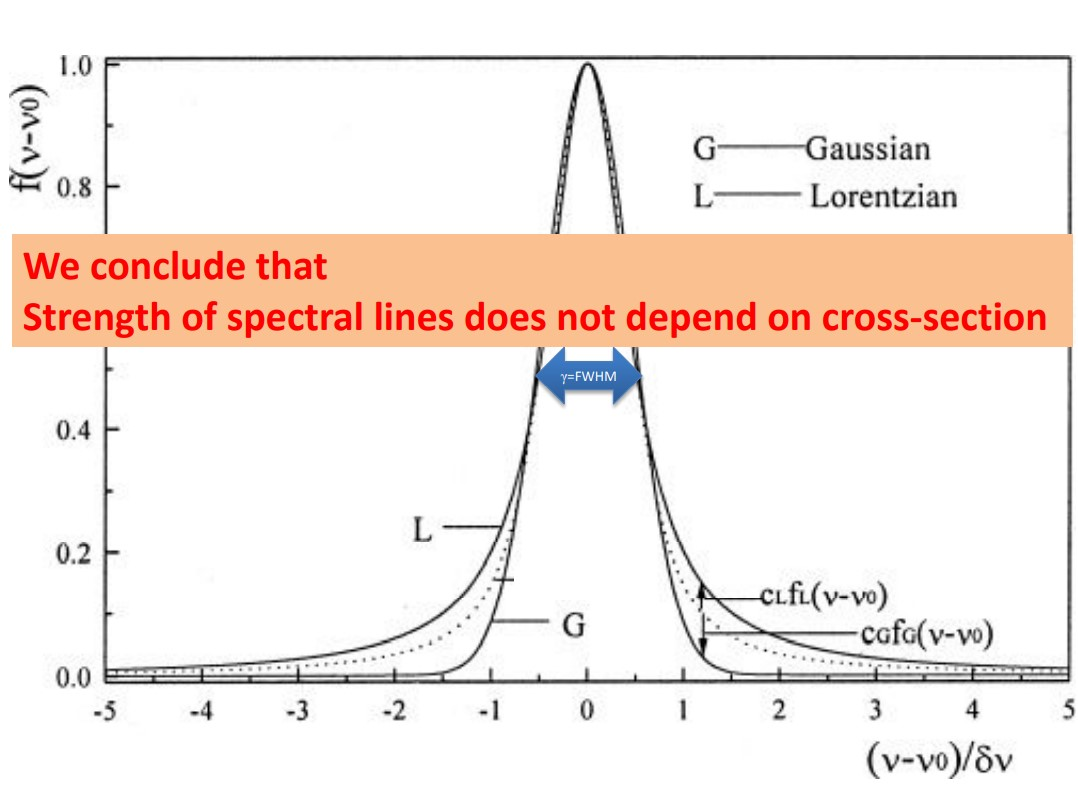
\includegraphics[width=8cm]{cross_section.jpg}
  \label{fig:cross section }
\end{figure}

Si evince che le righe spettrali non devono essere delte di Dirac, come a priori si potrebbe pensare avendo una sola transizione energetica. Se l'andamento fosse gaussiano, potremmo esprimerla in termini della $\sigma$, nel caso della lorentziana la $\sigma$ non esiste, però esiste la full width half maximum o larghezza a metà altezza (che, ad esempio, nella gaussiana vale 2.355$\sigma$).

Dalla corrispettiva sezione d'urto (cross section) deduciamo che non solo la frequenza del fotone può essere assorbita, ma anche frequenze vicine, secondo tale legge.

\subsubsection{Allargamento collisionale}

Finora abbiamo osservato atomi isolati, ma si tratta di un modello semplificato. Nella realtà, a questi processi vanno legati quelli collisionali: anche gli urti tra gli atomi possono trasferire un elettrone da un livello all'altro. Ricordiamo che l'urto non è necessariamente inteso come collisione ma come interazione: le cariche sentono una l'influenza dell'altra a causa del campo elettrico da esse generato.

Le collisioni posso essere di due tipi:

\begin{itemize}
  \item Collisione che porta da un livello basso ad un livello alto;
  \item Collisioni super elastiche: in questo tipo di interazione, piuttosto che diminuire l'energia aumenta.
\end{itemize}

\comment{Ciò che ci interessa ricordare è che il processo di popolazione di un livello dipende:

\begin{itemize}
  \item Dalle proprietà atomiche;
  \item Dal campo di radiazione;
  \item Dall'ambiente in termini di collisioni.
\end{itemize}}

Cosa accade alla radiazione quando viene emessa da emettitori che collidono? Nell'approssimazione che l'emettitore sia un oscillatore armonico smorzato, esso ha campo elettrico

\begin{equation*}
  E(t)=Ae^{-\beta t} \cos{(2\pi \nu_0 t - \phi)}
\end{equation*}

dove $A$ e $\phi$ sono l'ampiezza e la fase dell'oscillazione.

L'effetto delle collisioni con gli elettroni (o altre particelle cariche presenti nel mezzo) può essere schematizzato pensando che le collisioni siano dei processi che avvengano istantaneamente (approssimazione d'impatto) e che ciascuna collisione introduca nel campo elettrico emesso dall'atomo uno sfasamento di ampiezza aleatoria. Per effetto delle collisioni il campo elettrico è quindi descritto dalla funzione

$$E(t)=Ae^{-\beta t} \cos{[2\pi \nu_0 t - \phi(t)]}$$

Per descrivere l'effetto delle collisioni, Weisskopf ipotizzò che, a causa degli urti, l'emettitore avrà una fase iniziale diversa da quella standard che avrebbero tutti gli emettitori che non collidono. Quindi a causa delle collisioni, che sono casuali, avremo una fase che dipende da $t$; l'effetto di questa variazione di fase è che $E(t)$ invece di essere smorzata dal coefficiente $e^{-\beta t}$, ogni tanto fa dei "salti" di fase\footnote{Per essere rigorosi il motivo è che $\phi(t)$ è una funzione a carattere stocastico che presenta delle discontinuità in corrispondenza di ciascun istante in cui si verifica una collisione.}. Per capire allora a quali frequenze emetterebbero, Weisskopf sfruttò le trasformate di Fourier che permettono di passare dal tempo alle frequenze:

$$\hat{E}(\nu)=\frac{1}{2\pi}\int_{-\infty}^{\infty} E(t) e^{2 \pi i\nu t} \,dt$$

andando a sostituire l'espressione di $E(t)$ otteniamo

$$\hat{E}(\nu)=\frac{A}{4\pi}\int_{0}^{+\infty} e^{2\pi i(\nu-\nu_0)t-\beta t+i \phi(t)}\, dt$$

Poiché vogliamo conoscere l'energia rimossa al campo di radiazione, che è uguale alla potenza emessa dall'oscillatore smorzato, calcoliamo il modulo quadro del campo:

\begin{equation*}
  |\hat{E}(\nu)|^2=\frac{A^2}{16 \pi^2}\int_{0}^{+\infty}\, dt_1 \int_{0}^{+\infty}dt_2 \, e^{2\pi i(\nu-\nu_0)(t_1-t_2)-\beta (t_1-t_2)+i [\phi(t_1)-\phi(t_2)]}
\end{equation*}

Nota: si deve prendere il complesso coniugato, perché $E^2=E^*E$.

\hrulefill

Riportiamo i \textsc{calcoli astromeccanici} necessari ad arrivare al risultato finale.

\begin{figure}[H]
  \centering
  \begin{tikzpicture}[scale=2]
    \draw[->] (0,-0.2) -- (0,2);
    \draw[->] (-0.2,0) -- (2,0);
    \draw (0,0) -- (1.5,1.5);
    \node at (0.5,1) {A};
    \node at (1,0.5) {B};
  \end{tikzpicture}
\end{figure}

La regione A è quella in cui $t_1 < t_2$, mentre nella regione B si ha $t_2 < t_1$.

\vspace{0.2cm}La quantità $\Delta \phi=\Delta \phi(t_1) - \Delta \phi(t_2)$ ha carattere stocastico. Se durante l'intervallo di tempo che intercorre fra $t_1$ e $t_2$ (oppure fra $t_2$ e $t_1$) non avvengono collisioni, allora $\Delta \phi=0$, e si ha

\begin{equation*}
  e^{i\Delta \phi}=1
\end{equation*}

Se invece nello stesso intervallo avvengono molte collisioni, tenendo conto del fatto che le fasi introdotte dalle singole collisioni sono aleatorie, si ottiene, mediando su tutte le possibili “storie collisionali”,

\begin{equation*}
  e^{i\Delta \phi}=0
\end{equation*}

Se si indica quindi con $f$ la frequenza delle collisioni (numero di collisioni per unità di tempo), si può ragionevolmente assumere che valga la seguente approssimazione

\begin{equation*}
  e^{i\Delta \phi}=e^{-f|t_1 - t_2|}
\end{equation*}

Sostituendo questa espressione nell'integrale si ha quindi

\begin{equation*}
  |\hat{E}(\nu)|^2=\frac{A^2}{16 \pi^2}\int_{0}^{+\infty}\, dt_1 \int_{0}^{+\infty} dt_2\, e^{2\pi i(\nu-\nu_0)(t_1-t_2)-\beta (t_1-t_2)-f|t_1 - t_2|}
\end{equation*}

L'integrale doppio che compare in questa espressione si può calcolare distinguendo nel piano $(t1, t2)$ le due regioni A e B illustrate nella figura sopra. Osservando che l'integrale relativo alla regione B si può ottenere da quello relativo alla regione A cambiando di segno la quantità $\nu - \nu_0$, si ottiene

\begin{equation*}
  |\hat{E}(\nu)|^2=\mathcal{A} + \mathcal{B}
\end{equation*}

dove 

\begin{equation*}
  \mathcal{A}=\frac{A^2}{16 \pi^2}\int_{0}^{+\infty}\, dt_1 \int_{0}^{+\infty} dt_2\, e^{2\pi i(\nu-\nu_0)(t_1-t_2)-\beta (t_1-t_2)-f(t_2 - t_1)}
\end{equation*}

e dove $\mathcal{B}$ si ottiene da $\mathcal{A}$ mediante la sostituzione $(\nu - \nu_0) \to (\nu_0 - \nu)$. L'integrale doppio si calcola con metodi elementari e, aggiungendo $\mathcal{B}$ ad $\mathcal{A}$, si ottiene

\begin{equation*}
  |\hat{E}(\nu)|^2=\frac{A^2}{64 \pi^4} \frac{\gamma + 2f}{\gamma} \frac{1}{(\nu - \nu_0)^2 + \left( \frac{\gamma + 2f}{4 \pi} \right)^2}
\end{equation*}

e, ponendo

\begin{equation*}
  \Gamma=\frac{\gamma + 2f}{4 \pi}
\end{equation*}

si ottiene per il profilo normalizzato in frequenza l'espressione

\begin{equation*}
  \phi(\nu - \nu_0)=\frac{1}{\pi} \frac{\Gamma}{(\nu - \nu_0)^2 + \Gamma^2}
\end{equation*}

La funzione che descrive l'andamento del profilo con la frequenza è detta funzione di Lorentz (o funzione Lorentziana). La quantità $\Gamma$, detta costante di
smorzamento (o costante di \textit{damping}), contiene un contributo naturale e un contributo collisionale. Essa può essere posta nella forma

\begin{equation*}
  \Gamma=\Gamma_n + \Gamma_c
\end{equation*}

dove

\begin{equation*}
  \Gamma_n=\frac{\gamma}{4 \pi}
  \quad,\quad
  \Gamma_c=\frac{f}{4 \pi}
\end{equation*}

\hrulefill

La soluzione di tale integrale è ancora una funzione di Lorentz:

\begin{equation*}
  \phi(\nu - \nu_0)=\frac{1}{\pi} \frac{\Gamma}{(\nu - \nu_0)^2 + \Gamma^2}
\end{equation*}

Essa è un'emissione che ha lo stesso andamento funzionale dell'oscillatore smorzato, ciò che cambia è la costante di smorzamento $\gamma$, la quale risulta essere pari alla somma delle varie costanti. Nel caso dell'oscillatore semplice tale costante è data dall'indeterminazione dei livelli energetici, in questo caso è legata alla frequenza e alla quantità delle collisioni. Dunque l'emissione di un oscillatore ha andamento Lorentziano sia che sia solo, che in caso di collisioni, però la costante di smorzamento sarà diversa.

Il motivo per cui la rappresentazione delle righe spettrali nel caso in cui avvengano collisioni è ancora una lorentziana è che una convoluzione di Lorentziane è una lorentziana con larghezza diversa.

\comment{Consideriamo adesso il diagramma di Grotrian per l'H (diagramma che permette di visualizzare graficamente transizioni relative ad un livello energetico), e due atomi di H che collidono\footnote{in realtà le collisioni possono avvenire con qualunque cosa ma dato che l'H è l'elemento più abbondante è più probabile che avvengano con altri atomi di H}. Come i livelli energetici variano in funzione della distanza non è prevedibile, l'energia infatti talvolta può aumentare e altre volte diminuire in modo imprevedibile.

Immaginiamo ora un oggetto che si muove molto velocemente e ogni volta che si muove i suoi livelli energetici si modificano in funzione di ciò che ha vicino l'oggetto, sostanzialmente ogni volta che si muove emette una frequenza che è un po' diversa da quella imperturbata. La distribuzione delle frequenze emesse è rappresentabile con delle funzioni di Lorentz centrate sulla frequenza in cui è imperturbato e con una larghezza a metà altezza $\gamma$ che dipende dal numero di urti.



Detto ciò, esiste un'equazione che riassume quali sono le popolazioni dei livelli in funzione di un solo parametro, nel caso di quello che è chiamato equilibrio termodinamico, che è la temperatura. Sappiamo che di norma possiamo descrivere l'ambiente in funzione della sua temperatura, ma non è detto che la temperatura delle componenti di questo ambiente sia la stessa. Consideriamo il caso di protoni ed elettroni: non è detto che la velocità degli elettroni sia relazionata alla velocità dei protoni come si può desumere dalla conservazione della quantità di moto: la situazione potrebbe essere più complicata. Tuttavia, in un ambiente caratterizzato da un grandissimo numero di collisioni si può arrivare alla condizione di equilibrio termodinamico, nella quale tutti i processi sono all'equilibrio e sono rappresentati dallo stesso valore di temperatura. Boltzmann mostrò che in questo caso, dati due livelli in un atomo, il rapporto di popolazione dei due livelli $A$ e $B$ è dato dalla seguente equazione: 

$$\frac{N_A}{N_B} = \frac{g_A}{g_B} e^{\frac{-(E_A-E_B)}{kT}}$$

In cui figurano delle costanti $g_{A/B}$ dipendenti dal livello (dette peso statistico) e la legge esponenziale con il rapporto tra l'energia dei due livelli e la temperatura in Kelvin ad esponente. Con questa equazione di Boltzmann diventa tutto facile.

Questa equazione è intuibile in quanto all'aumentare della temperatura aumentano le collisioni e di conseguenza avremo più stati eccitati. Un caso limite potrebbe essere rappresentato dalla temperatura infinita; in questo caso il rapporto di popolazione dei livelli diventa una costante ed entreranno in gioco le sole proprietà dell'atomo. Al contrario, se la temperatura è molto bassa, pochi saranno i livelli eccitati.}

\subsubsection{Allargamento Doppler}

Come abbiamo detto, esiste un'ulteriore causa di allargamento del coefficiente di emissione (o di assorbimento) dovuta all'agitazione termica degli atomi.

Considerato un gas, è comune dire che la distribuzione delle velocità delle particelle che lo compongono è Maxwelliana. Non si tratta quindi di un moto ordinato e le particelle presentano una velocità media che dipende dalla temperatura che, se il sistema è in equilibrio termodinamico, sarà la stessa temperatura necessaria nell'equazione di Saha o di Boltzmann a stabilire la popolazione tra i livelli. 

Indichiamo con $P(w) dw$ la probabilità che la componente della velocità dell'atomo lungo la direzione della radiazione emessa sia compresa fra $w$ e $w + dw$. Tale probabilità si può esprimere nella forma

\begin{equation*}
  P(w)=\frac{1}{\sqrt{\pi} w_T} e^{-(w/w_T)^2}
\end{equation*}

dove abbiamo introdotto la velocità termica $w_T$ definita dall'equazione

\begin{equation*}
  w_T=\sqrt{\frac{2 k_B T}{M}}
\end{equation*}

essendo $M$ la massa dell'atomo. Per effetto Doppler, un atomo che si muova con la componente di velocità $w$ presenta (all'ordine relativistico pià basso) un profilo di emissione centrato intorno alla frequenza $\nu_0'$ data da

\begin{equation*}
  \nu_0'=\nu_0 \left( 1 + \frac{w}{c} \right)
\end{equation*}

Ci aspettiamo di vedere che il coefficiente di assorbimento della transizione legato-legato, che è la funzione di Lorentz, somma di tutte le lorentziane convoluta con il profilo dell'andamento delle velocità, sia la somma di tutti i possibili profili shiftati ognuno in lunghezza. Cerchiamo di spiegare meglio questo concetto

Questi atomi che emettono non sono fermi, e nel loro profilo e nel loro modo di emettere ci deve essere traccia di come effettivamente si stanno muovendo. Per come abbiamo visto le cose fino ad adesso il profilo è comunque lorentziano, sia che sia l'allargamento naturale sia che sia prodotto da collisioni. Questa forma però si perde quando si tiene in considerazione il fatto che gli emettitori sono in movimento. Il profilo di Lorentz infatti è un profilo che viene prodotto nel sistema di riferimento dell'emettitore, quindi esso vede quella frequenza come utile per la transizione e riemette questa nel suo sistema di riferimento, però in realtà l'emettitore può avere una velocità rispetto all'osservatore. Se ad esempio abbiamo un atomo che emette nella sua frequenza naturale di transizione che si muove verso di noi, vedremo la riga spostata verso il blu per effetto doppler.

Se siamo in presenza di un campo di radiazione e abbiamo una serie di emettitori che si muovono in tutte le direzioni all'interno di un certo volume, essi percepiranno la frequenza dei fotoni in arrivo in maniera diversa, in funzione della loro velocità rispetto al campo di radiazione; ciò vuol dire che per esempio non assorbiranno esattamente solo la riga della H-$\alpha$, ma anche frequenze un po' diverse tali che vengano percepite nel loro sistema di riferimento come delle H-$\alpha$.

In altre parole, il profilo di una riga spettrale, che abbiamo descritto con una lorentziana, prevederà rispetto alla frequenza di laboratorio, un doppler shift.

%Il profilo comunque rimane ancora di tipo lorentziano però, quello che percepisce l'osservatore è legato alla distribuzione della velocità degli emettitori o degli assorbitori, quindi quello che importa è la velocità degli emettitori proiettata nella direzione di osservazione. In altre parole l'importante non è la velocità dell'oggetto in generale, ma la proiezione della velocità nella direzione di osservazione.

%Questa direzione di osservazione in astronomia la troviamo sotto il nome di line of sight o line of view (linea di vista).

%Facciamo delle considerazioni. Abbiamo visto che gli atomi si muovono e questo può cambiare il profilo della riga. Il comportamento medio non tiene conto del fatto che gli assorbitori si stanno muovendo, cioè quello che abbiamo visto prima discutendo di collisioni parlava implicitamente di velocità. Però in realtà non abbiamo incluso nessuna forma di effetto doppler nell'argomento precedente: lo stesso scenario che abbiamo descritto si potrebbe ottenere con un emettitore fermo che viene colpito, perché le collisioni sono gli altri che gli vengono addosso, però anche lui in realtà si sta muovendo, però in quella rappresentazione precedente, per cui siamo giunti ancora una profilo di Lorentz, noi non abbiamo incluso i campi di velocità dell'emettitore. A questo punto dobbiamo chiederci come si muovono gli emettitori in un in un plasma.

%Riprendendo la definizione della distribuzione maxwelliana delle velocità, cioè se ho una serie di particelle che tra di loro collidono, in un volume chiuso, possiamo descrivere tutte le velocità di questi oggetti sulla base di un valore medio che è dato dal

%\textbf{sta formula non la so}

%$$\xi= \sqrt{\frac{2KT}{m}}$$

%Questo è un parametro molto importante per noi, perché significa che la varianza della distribuzione velocità Maxwelliana cambia da elemento ad elemento, quindi per dedurre le velocità nel plasma dobbiamo sapere di cosa è fatto.

%Come ci aspettiamo sia il profilo finale di questa emissione?
Ogni atomo emette una lorentziana, la quale è spostata in velocità di una certa quantità (quindi è shiftata di fatto) e il profilo finale sarà la somma di tutte queste lorentziane shiftate. Quello che bisogna sapere è quanti sono gli atomi shiftati di una certa quantità, e ciò è dato dalla probabilità della maxwelliana. In particolare secondo la distribuzione maxwelliana avremo molti atomi che sono apparentemente fermi, man mano che ci allontaniamo in velocità ne avremo sempre meno. Il risultato finale è allora semplicemente l'integrale sul campo di velocità.

Quali sono le forme tipiche di queste distribuzioni di Maxwell? Sono curve asimmetriche (perché ovviamente non ci sono velocità negative), con un picco che dipende dalla temperatura.

In definitiva, il profilo di emissione dovuto all'insieme degli atomi è quindi dato da

\begin{equation*}
  \varphi(\nu - \nu_0)=\int_{-\infty}^{+\infty} \frac{1}{\pi} \frac{\Gamma}{(\nu - \nu_0 - \nu_0 w/c)^2 + \Gamma^2} \frac{1}{\sqrt{\pi} w_T} e^{-(w/w_T)^2} \, dw
\end{equation*}

Per il calcolo effettivo necessario a caratterizzare il profilo, si introducono una serie di coefficienti, di cui uno si chiama \textit{allargamento doppler della riga} o Doppler width of the line $\Delta \nu_D$:


$$\Delta \nu_D=\frac{\nu_0 w_T}{c}$$

Avendo introdotto tale parametro, possiamo esprimere la distanza (in frequenza) $v$ dalla frequenza centrale in funzione di esso, come

$$v=\frac{\nu - \nu_0}{\Delta \nu_{D}}$$

Se inoltre introduciamo il cambiamento di variabili

$$y=\frac{\Delta \nu}{\Delta \nu_{D}}=\frac{w}{w_T}$$

ed il coefficiente di smorzamento $a$, definito come

$$a=\frac{\gamma}{4 \pi \Delta \nu_{D}}$$

Allora il profilo risultante può essere espresso come

$$\varphi(\nu - \nu_0)=\frac{1}{\sqrt{\pi} \Delta\nu_D} H(a,v)$$

dove $H(a,v)$ è detta \textbf{funzione di Voigt} che ha forma:

$$H(a,v)=\frac{a}{\pi} \int_{-\infty}^{+\infty} \frac{e^{-y^2}}{(v-y)^2 + a^2} \; dy$$

Tale funzione rappresenta la forma delle righe spettrali prodotta da un gas in cui gli emettitori si muovono con una distribuzione Maxwelliana delle velocità. Essa può avere una larghezza diversa in funzione del parametro $a$.

Il profilo della riga spettrale non sarà più una lorentziana, ma assumerà la seguente forma:

\begin{figure}[h]
  \centering
  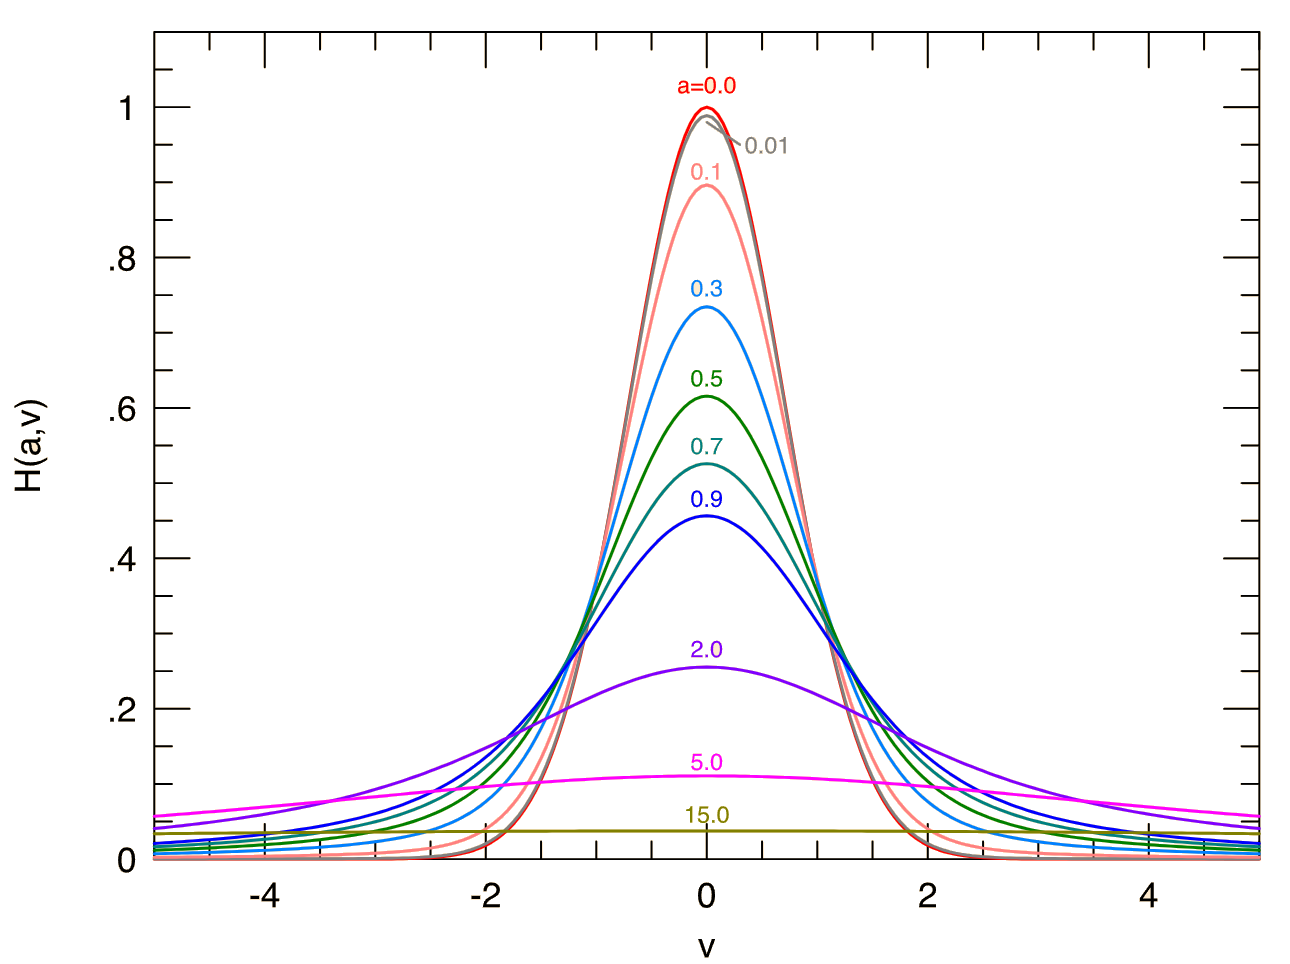
\includegraphics[width=8cm]{immagini/voigt_profile.png}
  \label{fig:voigtprofile}
\end{figure}

Tale curva non è caratterizzata da una costante di smorzamento, ma dalla velocità media delle particelle, quella che abbiamo chiamato Doppler width.

La funzione di Voigt gode di alcune proprietà che possono essere dedotte dalla sua espressione generale:

\begin{enumerate}
  \item $\displaystyle \int_{-\infty}^{+\infty} H(a,v) \; dv=\sqrt{\pi}$;
  \item $\displaystyle \lim_{a \to 0} H(a,v)=e^{-v^2}$;
  \item $\displaystyle \lim_{a \to \infty} H(v,a)=\frac{1}{\sqrt{\pi}} \frac{a}{v^2 + a^2}$
\end{enumerate}

La prima proprietà permette di dimostrare con facili trasformazioni che il profilo $\varphi(\nu - \nu_0)$ è normalizzato a 1 in frequenza

\begin{equation*}
  \int_{-\infty}^{+\infty} \varphi(\nu - \nu_0) \; d\nu=1
\end{equation*}

Le altre due proprietà mostrano che, nel caso limite di smorzamento trascurabile, la funzione di Voigt assume la forma Gaussiana, mentre, nel caso limite opposto, in cui l'allargamento termico è trascurabile, la funzione di Voigt degenera in una Lorentziana. In generale, la funzione di Voigt presenta un andamento Gaussiano intorno a $v=0$ e un andamento Lorentziano nelle ali.

In un profilo di Voigt possiamo osservare due andamenti: uno esponenziale nella parte centrale della riga (detto "core" della riga), uno come l'inverso di un polinomio $\frac{1}{(v-y)^2}$ ai lati, dove ricordiamo che $v$ è la differenza tra la frequenza e la frequenza centrale in unità di allargamento Doppler.

Il nostro obiettivo è di determinare questi parametri in funzione della temperatura e della massa delle particelle. Spesso allora è utile approssimare la funzione di Voigt con la seguente funzione

\begin{equation*}
  H(a,v)=e^{-v^2}+\frac{a}{\sqrt{\pi}v^2}
\end{equation*}

In questo modo possiamo fittare un profilo osservato e misurare $a$. Da questo, nota $\gamma$ della transizione, troviamo la Doppler width. Da essa si calcola $w_T$ da cui si ricava facilmente la temperatura (cinetica) del plasma che si sta osservando, dato che sono note la velocità della luce e la frequenza. Se i calcoli sono corretti tale temperatura dovrà essere consistente con la temperatura efficace della stella e con le righe spettrali osservate.

\vspace{0.2cm}Bisogna però fare attenzione al fatto che si può avere effetto Doppler anche a causa dei dei moti turbolenti in certe regioni della stella. Si distinguono due casi:

\begin{itemize}
  \item \textbf{micro-turbolenza}: è il caso in cui le dimensioni della zona interessata sono comparabili con quelle del libero cammino medio dei fotoni. In questo caso la larghezza doppler aumenta, essendoci il contributo della velocità della turbolenza:
  \begin{equation*}
    \Delta\nu_D=\frac{\nu_0}{c} \sqrt{\frac{2kT}{M} + v^2_{\rm turb}}
  \end{equation*}
  \item \textbf{macro-turbolenza}: è il caso in cui le dimensioni della zona maggiori di quelle del libero cammino medio dei fotoni. In questo caso il profilo di Voigt non muta, sarà soltanto spostato per intero con la stessa velocità delle bolle. Un esempio di tale condizione è quello delle bolle di gas sulla superficie solare, in cui le particelle che le costituiscono si muovono insieme in blocchi.
\end{itemize}

\subsubsection{Allargamento per pressione}

Gli orbitali di un atomo possono essere perturbati nella collisione con un atomo neutro o con l'interazione del campo elettrico di uno ione. La variazione in energia prodotta dalla collisione è funzione della distanza $r$ tra l'assorbitore e il perturbatore e può essere approssimata dalla legge $\Delta E \sim k \cdot r^{-n}$, con $k$ costante. Da Essa segue che la variazione in frequenza è pari a

\begin{equation*}
  \Delta \nu=\frac{\Delta E}{h}=C_n r^{-n}
\end{equation*}

con $C_n$ coefficienti che si ricavano in laboratorio. In particolare:

\begin{itemize}
  \item Per $n=2$ si ha allargamento Stark lineare (H + particella carica).
  
  Esso si verifica tramite l'effetto Stark lineare, che deriva dall'interazione di un emettitore con un campo elettrico di una particella carica a una certa distanza $r$, causando uno spostamento in energia lineare rispetto alla forza del campo;
  \item Per $n=3$ si ha allargamento per risonanza (atomo A + atomo A).
  
  Esso si verifica quando la particella perturbante è dello stesso tipo della particella emittente, introducendo la possibilità di un processo di scambio di energia;
  \item Per $n=4$ si ha allargamento Stark quadratico (atomo non idrogenoide + particella carica)
  
  Esso si verifica tramite l'effetto Stark quadratico, che deriva dall'interazione di un emettitore con un campo elettrico, causando uno spostamento in energia quadratico rispetto alla forza del campo;
  \item Per $n=6$ si ha allargamento van der Waals (atomo A + atomo B).
  
  Esso si verifica quando la particella emittente è perturbata dalle forze di Van der Waals. Nel caso quasi statico, un profilo di Van der Waals è spesso utile per descrivere il profilo. Lo spostamento dell'energia in funzione della distanza tra le particelle interagenti è dato principalmente dalle ali del potenziale di Lennard-Jones.
\end{itemize}

L'effetto cumulativo è dato da

\begin{equation*}
  \varphi(\nu - \nu_0)=\int_{0}^{+\infty} C_n r^{-n}
\end{equation*}


Quello riportato in figura è in una simulazione numerica (in rosso) di uno spettro stellare (in nero). Si possono vedere che tutte le righe, sia quelle piu sottili che quelle più larghe, che sono quelle con il $\gamma$ maggiore, sono perfettamente riprodotte.
Questo significa che guardando questa stella in nero e facendo lo spettro teorico, possiamo dire qual è la composizione chimica delle stelle.

%Di per sé ciò non è fondamentale, quello che è fondamentale è il quadro totale: la composizione chimica dell'universo, come evolve, perché cambia come cambia ecc.

\begin{figure}[H]
  \centering
  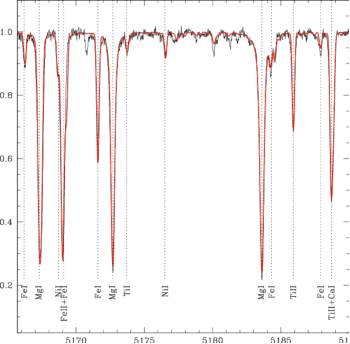
\includegraphics[width=0.5\linewidth]{graficorossonero}
%\caption[Figura 1]{	n = 4 quadratic Stark effect}
\label{fig:graficorossonero}
\end{figure}

Quanto sono grandi queste righe? Ad esempio, la riga dell'idrogeno alfa, per effetto delle collisioni in una stella (che può essere il Sole), ha una full with maximum, cioè la sua larghezza a metà altezza, pari a mezzo Angstrom.

\E chiaro che tutto viene usato al rovescio, cioè prima misuriamo mezzo angstrom e poi misuriamo il numero di collisioni, quindi stabiliamo la densità.

\begin{figure}[H]
  \centering
  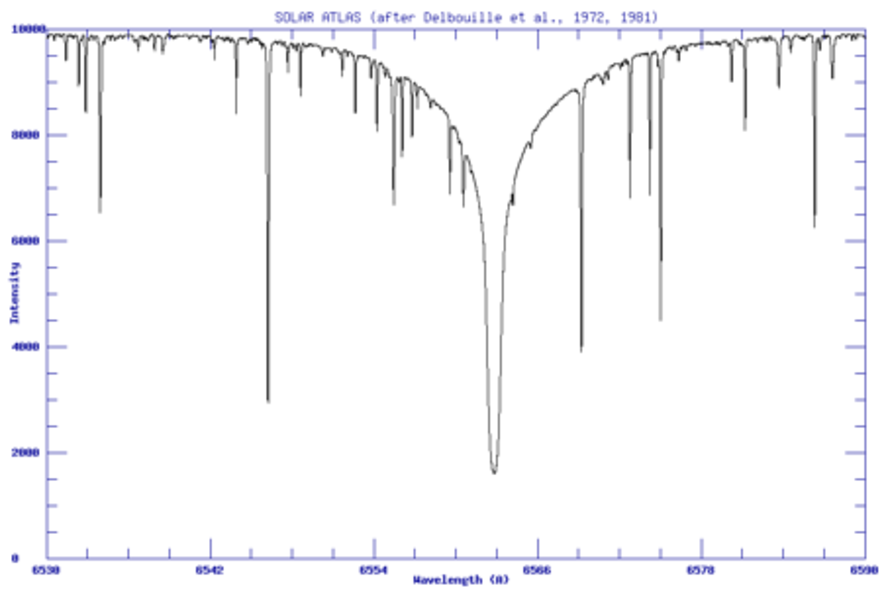
\includegraphics[width=0.5\linewidth]{linearstark}
  %\caption[Figura 1]{Full Width Half Maximum}
  \label{fig:linearstark}
\end{figure}

Ma perché abbiamo oggetti con righe di larghezza così diversa?

Prendendo in considerazione il diagramma HR, quello che osserviamo, sulla base della relazione tra luminosità e temperatura efficace, è un aumento del raggio delle stelle dal basso verso l'alto: le stelle in alto hanno un raggio molto più grande di quello delle stelle che si trovano più sotto, e siccome la densità è inversamente proporzionale al raggio segue che la densità degli oggetti in alto è molto piccola, mentre man mano che si va giù aumenta. Se ciò è vero, ci aspettiamo un incremento del numero di collisioni (che va con la densità) andando verso il basso. In conseguenza a ciò, ci aspettiamo righe spettrali molto strette e poche collisioni (quindi poco allargamento) per le stelle che sono in alto nel diagramma HR, che noi abbiamo definito di grande raggio, e questo è naturale in ambiente rarefatto perché le possibilità di collisione sono basse. Quindi le righe spettrali delle giganti, quelle che si trovano in alto nel diagramma, sono molto sottili. Man mano che si va giù verso la sequenza principale, il numero di collisioni aumenta e le righe spettrali diventano sempre più grandi.

Questo ci porta al concetto di luminosità, cioè noi non possiamo identificare una stella solo sulla base della temperatura, ma anche sulla base della sua gravità, ma storicamente questo concetto è stato chiamato luminosità. Si parla allora di \textit{classi di luminosità}.

All'interno della stessa classe spettrale esistono differenze negli allargamenti collisionali delle righe. A parità di tipo spettrale, stelle più luminose (e siccome $L=4\pi R^2 \sigma T_{\rm eff}^4$, stelle più grandi) mostrano righe più strette. Infatti, l'allargamento collisionale delle righe dipende dalla pressione alla superficie della stella, e questa dalla gravità superficiale $g = GM_*/R^22$. Stelle più grandi hanno una gravità superficiale minore, e quindi allargamento collisionale minore. Le classi spettrali così ottenute vengono chiamate classi di luminosità ed indicate con numeri romani da I (le più luminose, cioè quelle con allargamento minore) a V

Abbiamo la classe spettrale, che è legata alla presenza di righe dello spettro e la classe di luminosità che invece si relaziona al raggio.

La nomenclatura rimasta definisce le stelle della sequenza principale di classe quinta e man mano che si sale si va a classe quattro sulle super giganti, classe tre le giganti. 
Questo andamento della classe di luminosità adesso ha un senso non soltanto in termini di raggio, ma sulla base della densità della materia, cioè questi ambienti super giganti, sono praticamente ambienti rarefatti. 

\vspace{0.2cm}L'ultima cosa che possiamo imparare dalle righe spettrali su plasmi sono le macro-velocità, campi di velocità più ampi di quelli delle singole particelle. L'esempio tipico è la misura della velocità di rotazione di una stella sulla base delle righe spettrali emesse.

Per un rotatore rigido, come le stelle, è semplice ricavare la velocità di rotazione attorno ad un asse di rotazione fisso di ogni punto della sfera misurando il periodo: $v=C\frac{R}{T}$ (attenzione alla costante che dipende dalle unità di misura, solitamente $v$ si misura in km/s, $R$ in raggi solari e $T$ in giorni; per il Sole ad esempio C=50.6).

Nel nostro caso abbiamo bisogno di misurare la  componente della velocità nella direzione di osservazione che chiamiamo $z$. Si tratta sostanzialmente di una proiezione di un angolo di inclinazione $i$ (angolo tra l'asse di rotazione e la direzione di osservazione della stella). Questa velocità radiale quindi risulta

$$v_r=x \, \Omega \sin{i}$$

con $\Omega$ velocità di rotazione, $x$ distanza dall'asse. Per cui il Doppler shifting diventa

$$\Delta \lambda=\frac{\lambda_0}{c} x \, \Omega \sin{i}$$

Ma come si misura questa velocità nella pratica? Quando osserviamo il disco visibile di una stella dividiamo questo in striscette verticali e calcoliamo il profilo di Voigt teorico di ciascuna di esse al variare della velocità di rotazione. Sommando i contributi di tutte le strisce otteniamo il profilo di Voigt complessivo che approssima tanto meglio quello ricavato dall'osservazione delle righe spettrali del disco quanto più la proiezione della velocità di rotazione della stella si avvicina a quella reale.